%%%%%%%%%%%%%%%%%%%%%%%%%%%%%%%%%%%%%%%%%%%%%%%%%%%%%%%%%%%%%%%%%%%%%%%%
%    INSTANTIATE YOUR DOCUMENT CLASS WITH THE ECAI OPTION.
%    For final camera-ready copy, replace 'report' with 'final'.
%%%%%%%%%%%%%%%%%%%%%%%%%%%%%%%%%%%%%%%%%%%%%%%%%%%%%%%%%%%%%%%%%%%%%%%%
\documentclass[final]{ecai} 
%\documentclass[doubleblind]{ecai} 
\usepackage{times}
\usepackage{graphicx}
\usepackage{latexsym}
\usepackage{amsmath}
\usepackage{amssymb}
\usepackage{url}
\usepackage{hyperref}
\usepackage{natbib}
\usepackage{multirow}
\usepackage{tcolorbox}
\tcbuselibrary{listingsutf8}


\begin{document}

\begin{frontmatter}

%%%%%%%%%%%%%%%%%%%%%%%%%%%%%%%%%%%%%%%%%%%%%%%%%%%%%%%%%%%%%%%%%%%%%%%%
%    TITLE SECTION
%%%%%%%%%%%%%%%%%%%%%%%%%%%%%%%%%%%%%%%%%%%%%%%%%%%%%%%%%%%%%%%%%%%%%%%%
\title{Team21 - Entity Matters: A Comparative Study of Machine Translation Fidelity in Large Language Models}

%%%%%%%%%%%%%%%%%%%%%%%%%%%%%%%%%%%%%%%%%%%%%%%%%%%%%%%%%%%%%%%%%%%%%%%%
%    AUTHOR SECTION
%%%%%%%%%%%%%%%%%%%%%%%%%%%%%%%%%%%%%%%%%%%%%%%%%%%%%%%%%%%%%%%%%%%%%%%%
\author{\fnms{Aastik}~\snm{Shrivastava}}
\author{\fnms{Abhitosh}}
\author{\fnms{Amit}~\snm{Nitin Joshi}}
\author{\fnms{Ayush}~\snm{Ravindra Jha}}
\author{\fnms{Raghavendra}~\snm{Naik}}
\author{\fnms{Sibashis}~\snm{Kumar Sahu}}

%%%%%%%%%%%%%%%%%%%%%%%%%%%%%%%%%%%%%%%%%%%%%%%%%%%%%%%%%%%%%%%%%%%%%%%%
%    ABSTRACT SECTION

%%%%%%%%%%%%%%%%%%%%%%%%%%%%%%%%%%%%%%%%%%%%%%%%%%%%%%%%%%%%%%%%%%%%%%%%
\begin{abstract}
Translation of named entities is challenging for traditional machine translation systems, as there may be cultural 
or domain-specific references that may not be easily translated. 
This impacts the effectiveness of such systems in real-world scenarios. 
We draw inspiration from the SemEval 2025 Task 2 on Entity-Aware Machine Translation for this paper. 
The task was to translate an input sentence containing named entities from English to multiple target languages. 
In this paper, we attempted the task using various techniques and present our findings. 
We evaluated a range of open and closed-source models using various techniques, including prompt engineering, named entity recognition, and retrieval-augmented generation, 
to assess and improve their performance on the task.
We used Crosslingual Optimized Metric for Evaluation of Translation (COMET)\cite{rei-etal-2020-comet}
and Manual Entity Translation Accuracy (M-ETA) as metrics for evaluation of the quality of translation generated by these systems.
\end{abstract}
\end{frontmatter}

%%%%%%%%%%%%%%%%%%%%%%%%%%%%%%%%%%%%%%%%%%%%%%%%%%%%%%%%%%%%%%%%%%%%%%%%
%    MAIN BODY OF THE PAPER
%%%%%%%%%%%%%%%%%%%%%%%%%%%%%%%%%%%%%%%%%%%%%%%%%%%%%%%%%%%%%%%%%%%%%%%%

%%%%%%%%%%%%%%%%%%%%%%%%%%%%%%%%%%%%%%%%%%%%%%%%%%%%%%%%%%%%%%%%%%%%%%%%
%    Introduction
%%%%%%%%%%%%%%%%%%%%%%%%%%%%%%%%%%%%%%%%%%%%%%%%%%%%%%%%%%%%%%%%%%%%%%%%
\section{Introduction}
\label{sec:intro}
The accurate and contextually appropriate translation of named entities remains a formidable challenge
for conventional machine translation systems, as these specific linguistic elements often lack direct
lexical equivalents in target languages. This necessitates a sophisticated comprehension of their real-world
referents and inherent semantic roles. This persistent difficulty underscores the critical importance of Entity-Aware
Machine Translation (EA-MT). EA-MT represents a significant advancement, empowering machine translation systems to actively
recognize, classify and leverage an entity's specific type and attribute. By integrating this nuanced entity intelligence, 
EA-MT can effectively resolve ambiguities, ensure consistent rendering across diverse linguistic contexts, 
and generate translations that are not only grammatically sound but also factually precise, 
thereby critically enhancing the overall fidelity and trustworthiness of machine-generated content
 in sensitive and high-stakes applications.

%%%%%%%%%%%%%%%%%%%%%%%%%%%%%%%%%%%%%%%%%%%%%%%%%%%%%%%%%%%%%%%%%%%%%%%%
%    Related Work
%%%%%%%%%%%%%%%%%%%%%%%%%%%%%%%%%%%%%%%%%%%%%%%%%%%%%%%%%%%%%%%%%%%%%%%%

\section{Related Work}
\label{sec:related}
Our work builds upon several key advancements in machine translation and large language models. 
The field of machine translation was revolutionized by the introduction of Neural Machine Translation (NMT), 
particularly with the advent of the Transformer architecture \cite{vaswani2017attention}, 
which replaced recurrent and convolutional models with a purely attention-based mechanism, 
setting a new standard for performance.
More recently, Large Language Models (LLMs) have demonstrated remarkable capabilities in translation, 
often in a zero-shot or few-shot setting \cite{brown2020language}. 
Models pretrained on vast text corpora using a unified text-to-text framework, 
such as T5 \cite{raffel2020exploring}, have shown that a single model can be effectively prompted 
to perform a wide range of NLP tasks, including high-quality translation without task-specific fine-tuning.
A significant challenge in machine translation is the correct rendering of named entities,
which often carry critical semantic weight. This has been a long-standing area of research, 
with various approaches proposed to make NMT systems more "entity-aware." 
Early work focused on integrating external knowledge or explicitly marking entities to guide the translation process. 
These methods aim to improve translation fidelity by preventing entities from being misinterpreted 
as common words or being transliterated incorrectly.
To further enhance the contextual understanding of LLMs for specialized tasks, 
Retrieval-Augmented Generation (RAG) has emerged as a powerful technique \cite{lewis2020retrieval}. 
By retrieving relevant documents or knowledge snippets and providing them as context to the generator model, 
RAG has been successfully applied to knowledge-intensive NLP tasks. Its application to machine translation is 
particularly promising for handling domain-specific terminology and entities, 
as it allows the model to ground its translations in factual, retrieved data
a principle that underpins our RAG-based experiments with Wikidata. 
Finally, for evaluation, we rely on established metrics like COMET \cite{rei-etal-2020-comet}, 
a reference-based metric that leverages cross-lingual pretrained models to achieve high correlation
with human judgments of translation quality, and M-ETA,
which specifically measures the accuracy of entity translation in machine-generated text.

\section{Datasets}
\label{sec:datasets}

\begin{table}[h!]
\centering
\begin{tabular}{ll@{\hspace{8mm}}ll}
\hline
\textbf{Language} & \textbf{Train} & \textbf{Valid} & \textbf{Test} \\
\hline
Italian & 3,739 & 730 & 5,097 \\
Spanish & 5,160 & 739 & 5,337 \\
French & 5,531 & 724 & 5,464 \\
German & 4,087 & 731 & 5,875 \\
Arabic & 7,220 & 722 & 4,546 \\
Japanese & 7,225 & 723 & 5,107 \\
Chinese & - & 722 & 5,181 \\
Korean & - & 745 & 5,081 \\
Thai & - & 710 & 3,446 \\
Turkish & - & 732 & 4,472 \\
\hline
\textbf{Total} & \textbf{32,962} & \textbf{7,278} & \textbf{49,606} \\
\hline
\end{tabular}
\caption{Dataset distribution across languages}
\label{tab:dataset_distribution}
\end{table}

The datasets used in this study are derived from the SemEval 2025 Task 2 on Entity-Aware Machine Translation.
All sets, except for the blind test set, included English source texts and their translations in ten 
different languages - Italian, Spanish, French, German, Arabic, Japanese, Chinese, Korean, Thai, and Turkish. 
Each data entry typically featured an English sentence, at least one translation in a target language, 
and a relevant Wikidata ID. 
For example, an English query like "What year was The Great Gatsby published?" 
would be linked to its Korean translation and the Wikidata ID Q214371. We also referred the mintaka\cite{sen-etal-2022-mintaka} dataset,
high-quality knowledge base of Wikidata facts, primarily used for question answering. It can be used to create
datasets for fine-tuning Named Entity Recognition (NER) models.

%%%%%%%%%%%%%%%%%%%%%%%%%%%%%%%%%%%%%%%%%%%%%%%%%%%%%%%%%%%%%%%%%%%%%%%%
%    Methodology
%%%%%%%%%%%%%%%%%%%%%%%%%%%%%%%%%%%%%%%%%%%%%%%%%%%%%%%%%%%%%%%%%%%%%%%%
\section{Methodology}
\label{sec:methodology}
Our experimental methodology evaluated open-weight and closed-source Large Language Models (LLMs) on the SemEval 2025 Task 2 Entity-Aware Machine Translation (EA-MT) task. 
We explored direct translation through various prompting strategies and enhanced these with Retrieval-Augmented Generation (RAG)-inspired pipelines, focusing on robust named entity handling.

For direct translation, we established a baseline for open-weight models (e.g., Gemma, Llama, Mistral) and closed-source models (Google's Gemini-2.0-Flash and OpenAI's GPT-4o). 
\textbf{Zero-shot Translation} evaluated baseline fluency, often struggling with named entity recognition. \textbf{Few-shot Translation} used limited in-context examples to guide models, 
showing modest improvements despite prompt complexity challenges. \textbf{Chain-of-Thought (CoT) Prompting} was applied to closed-source models, instructing intermediate reasoning 
steps to enhance logical processing and entity handling. Prompt templates varied to include direct translation, prepended examples for few-shot, and reasoning guidance for CoT.

To mitigate named entity translation challenges, we implemented RAG-inspired pipelines. For open-weight models, this involved an LLM-based zero-shot NER approach 
(or spaCy for non-prompt-amenable models like NLLB), followed by prompt-based verification, deduplication, and Wikidata linking for accurate translations.
Key enhancements like \textbf{Entity Merging and Type Filtering} improved lookup precision and reduced ambiguity. Translated entities augmented 
the final translation prompt, incorporating a retry mechanism for fidelity. With Gemini-2.0-Flash, a similar spaCy-based \textbf{RAG-guided translation} approach 
was successfully attempted. This multi-faceted methodology enabled comprehensive evaluation of both direct translation and external knowledge 
integration's impact on EA-MT across contemporary LLMs.

\begin{figure}[h!]
    \centering
    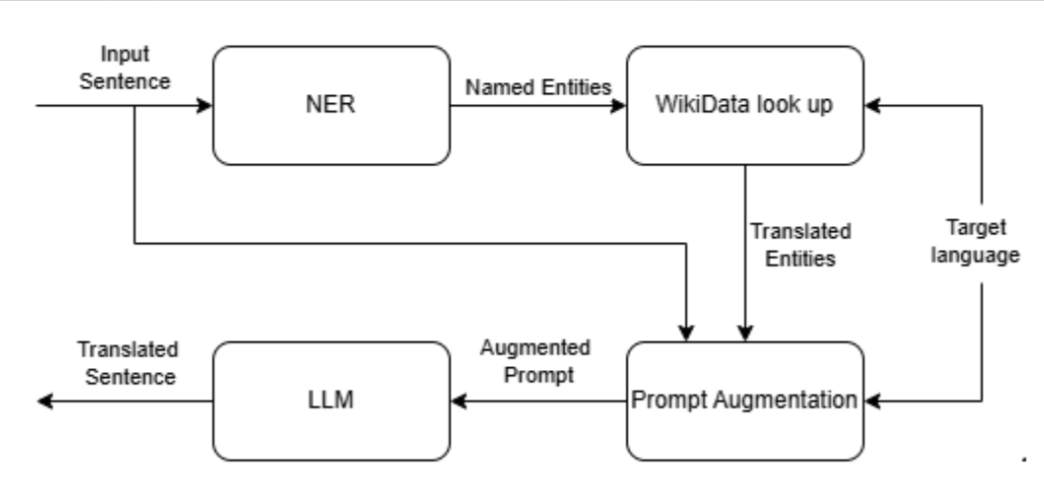
\includegraphics[width=1.0\linewidth]{rag.png}
    \caption{Illustration of the entity-aware RAG translation pipeline.}
    \label{fig:entity_pipeline}
\end{figure}

%%%%%%%%%%%%%%%%%%%%%%%%%%%%%%%%%%%%%%%%%%%%%%%%%%%%%%%%%%%%%%%%%%%%%%%%
%    Evaluation
%%%%%%%%%%%%%%%%%%%%%%%%%%%%%%%%%%%%%%%%%%%%%%%%%%%%%%%%%%%%%%%%%%%%%%%%
\section{Evaluation}
\label{sec:experiments}
Our system evaluations were conducted using the metrics specified for the shared task: COMET 
(Crosslingual Optimized Metric for Evaluation of Translation)\cite{rei-etal-2020-comet} and 
Manual Entity Translation Accuracy (M-ETA). 
COMET is a machine translation evaluation metric that utilizes a pre-trained model to derive 
quality scores by comparing machine-generated outputs against human reference translations. 
M-ETA specifically quantifies the precision of entity translations within machine-translated text, 
calculated as the ratio of correctly translated entities against a gold standard.
To provide a comprehensive assessment, the overall performance score, presented in Equation \ref{eq:overall_score}, 
is computed as the harmonic mean of the COMET and M-ETA metrics. This combined metric ensures that systems are 
evaluated not only on their general translation quality but also on their ability to accurately translate named entities.
\begin{equation}
\label{eq:overall_score}
\text{Overall Score} = 2 \times \frac{\text{COMET} \times \text{M-ETA}}{\text{COMET} + \text{M-ETA}}
\end{equation}

%%%%%%%%%%%%%%%%%%%%%%%%%%%%%%%%%%%%%%%%%%%%%%%%%%%%%%%%%%%%%%%%%%%%%%%%
%    Results
%%%%%%%%%%%%%%%%%%%%%%%%%%%%%%%%%%%%%%%%%%%%%%%%%%%%%%%%%%%%%%%%%%%%%%%%
\section{Results}
\label{eq:results}

\begin{table}[h!]
\centering
\small % Using small font size for compactness
\label{tab:combined_methods_avg_scores}
\begin{tabular}{|l|c|c|c|}
\hline
\textbf{Method:Model-Attempt} & \textbf{M-ETA} & \textbf{COMET} & \textbf{Overall Score} \\
\hline
RAG:gemma3\_4b & 66.52 & 91.12 & 76.79 \\
RAG:gemini-2.0-flash & 59.99 & 90.62 & 72.16 \\
RAG:fb\_nllb\_200\_3.3b & 48.75 & 89.08 & 62.51 \\
RAG:fb\_nllb\_200\_3.3b & 48.95 & 89.12 & 62.79 \\
RAG:mistral7b & 54.68 & 82.12 & 65.42 \\
RAG:mistral7b & 12.63 & 76.27 & 20.01 \\
\hline
ZS:gemini-2.0-flash-0 & 46.57 & 91.10 & 61.49 \\
ZS:gemini-2.0-flash-1 & 45.58 & 90.37 & 60.45 \\
ZS:fb\_nllb\_200\_3.3b & 23.66 & 88.19 & 35.47 \\
ZS:gpt-4o-0 & 39.67 & 90.93 & 54.55 \\
ZS:gpt-4o-1 & 37.33 & 90.35 & 52.11 \\
ZS:gemma3\_4b & 21.02 & 87.85 & 33.10 \\
ZS:llama3.1\_8b-0 & 17.70 & 83.99 & 28.16 \\
ZS:llama3.1\_8b-1 & 16.44 & 79.07 & 26.09 \\
ZS:mistral7b & 12.88 & 76.19 & 20.31 \\
\hline
FS:gemini-2.0-flash & 46.45 & 90.91 & 61.38 \\
FS:gpt-4o & 22.87 & 61.48 & 30.34 \\
FS:llama3.1\_8b-0 & 17.59 & 79.88 & 27.76 \\
FS:llama3.1\_8b-1 & 14.41 & 76.73 & 22.71 \\
FS:llama3.1\_8b-2 & 14.52 & 75.79 & 23.25 \\
\hline
CoT:gemini-2.0-flash & 43.55 & 90.65 & 58.70 \\
CoT:gpt-4o & 39.58 & 90.73 & 54.40 \\
\hline
\end{tabular}
\caption{Average M-ETA, COMET and Overall (Harmonic Mean) scores across languages for various approaches and models.}
\end{table}

Among all evaluated approaches, Retrieval-Augmented Generation (RAG) with models like Gemma3 IT 4B 
and Gemini 2.0 Flash demonstrates the most effective performance for the Entity-Aware Machine Translation (EA-MT) task. 
These configurations consistently outperform zero-shot, few-shot, and chain-of-thought baselines in terms of both adequacy
and fluency. The strength of RAG lies in its ability to leverage retrieved external knowledge, allowing models to 
better handle the translation of named entities—particularly those requiring disambiguation or that lack sufficient 
in-context information. This grounding is crucial for EA-MT, where preserving entity fidelity is a core requirement.

In contrast, zero-shot and few-shot prompting with large models such as Gemini 2.0 Flash, GPT-4o, 
and Facebook's NLLB 3 perform moderately well but show reduced reliability, especially when translating unseen or 
ambiguous entities. LLaMA 3.1 8B and Mistral 7B underperform across setups, indicating limited capability without retrieval 
support.

Chain-of-thought (CoT) prompting with Gemini 2.0 Flash and GPT-4o yields slight gains in adequacy but does not 
close the gap with RAG-based systems. Additionally, enhanced prompting strategies (e.g., variations in prompt design) 
do not consistently improve performance and occasionally lead to regressions.

%%%%%%%%%%%%%%%%%%%%%%%%%%%%%%%%%%%%%%%%%%%%%%%%%%%%%%%%%%%%%%%%%%%%%%%%
%    Future Work
%%%%%%%%%%%%%%%%%%%%%%%%%%%%%%%%%%%%%%%%%%%%%%%%%%%%%%%%%%%%%%%%%%%%%%%%
\section{Future Work}
\label{sec:future_work}
While RAG-based approaches with models like \textit{Gemma3 IT 4B} and \textit{Gemini 2.0 Flash} have shown strong performance, 
several directions can further enhance EA-MT systems. One promising path is fine-tuning models specifically for 
entity-aware translation, using annotated corpora or synthetic data that emphasize named entity handling. 
Techniques such as instruction tuning, LoRA-based adaptation, or reinforcement learning with entity-focused rewards 
can improve entity fidelity without requiring full retraining. 
Additionally, knowledge distillation from large models (e.g., \textit{Gemini} or \textit{GPT-4o}) into smaller, 
more efficient models offers a scalable way to preserve entity translation quality. On the retrieval side,
enhancements such as context-aware or cross-lingual retrieval—particularly those focused on entity-rich segments 
could improve grounding and reduce ambiguity. Incorporating entity tagging or canonicalization before translation, 
followed by post-generation substitution, may further reduce hallucinations. 
Finally, moving beyond adequacy and fluency, future work should adopt entity-aware evaluation metrics that explicitly 
assess correctness and faithfulness in named entity translation.
    

%%%%%%%%%%%%%%%%%%%%%%%%%%%%%%%%%%%%%%%%%%%%%%%%%%%%%%%%%%%%%%%%%%%%%%%%
%    Conclusion
%%%%%%%%%%%%%%%%%%%%%%%%%%%%%%%%%%%%%%%%%%%%%%%%%%%%%%%%%%%%%%%%%%%%%%%%
\section{Conclusion}
\label{sec:conclusion}
In this work, we evaluated a range of strategies for the Entity-Aware Machine Translation (EA-MT) 
task as part of SemEval 2025 Task 2. Our experiments demonstrate that Retrieval-Augmented 
Generation (RAG) methods, particularly those using high-capacity models like \textit{Gemma3 IT 4B} 
and \textit{Gemini 2.0 Flash}, substantially outperform zero-shot, few-shot, and chain-of-thought 
prompting approaches. RAG systems effectively leverage external knowledge to improve adequacy and 
fluency, especially in the translation of named entities.
We also observed that enhanced prompts and reasoning-based strategies, while helpful in certain 
cases, fall short of the gains achieved through retrieval. Our findings highlight the importance
of grounding language models in entity-relevant context to improve translation quality in 
multilingual settings.
This analysis establishes a strong foundation for further advancements in EA-MT. 
Future directions include targeted fine-tuning, knowledge distillation, improved retrieval 
strategies, and the development of entity-aware evaluation metrics. By integrating these 
improvements, we aim to build more accurate, robust, and deployable translation systems that 
are sensitive to entity correctness and cross-lingual consistency.


%%%%%%%%%%%%%%%%%%%%%%%%%%%%%%%%%%%%%%%%%%%%%%%%%%%%%%%%%%%%%%%%%%%%%%%%
%    BIBLIOGRAPHY SECTION
%%%%%%%%%%%%%%%%%%%%%%%%%%%%%%%%%%%%%%%%%%%%%%%%%%%%%%%%%%%%%%%%%%%%%%%%
\bibliography{references}

\clearpage
\renewcommand{\thesection}{A}
\renewcommand{\thesubsection}{A.\arabic{subsection}}

%%%%%%%%%%%%%%%%%%%%%%%%%%%%%%%%%%%%%%%%%%%%%%%%%%%%%%%%%%%%%%%%%%%%%%%%
%    Appendix
%%%%%%%%%%%%%%%%%%%%%%%%%%%%%%%%%%%%%%%%%%%%%%%%%%%%%%%%%%%%%%%%%%%%%%%%
\section{Appendix}

\subsection{Individual Contributions}

\textbf{Aastik Shrivastava}: Evaluated the \textit{Llama3.1\_8b} model employing zero-shot and few-shot prompting strategies, using simple 
and more detailed prompt designs. Also worked on performing entity recognition using SpaCy using post-porcessing techniques such as 
entity merging and normalization Identified entities were matched against Wikidata, with type-based filtering applied to improve precision and resolve ambiguities. 
Translations of entities were injected into the input prior to final sentence translation by NLLB model.

\textbf{Abhitosh}: Lead the project group. Identified the topic for project. Outlined an approach of experiments that every individual in the project can try out.
Evaluated \textit{Gemini-2.0-flash} model using one-shot, few-shot and chain-of-thought prompts. Optimized invocation of Gemini API to avoid encountering 
rate limits for evaluations, which facilated evaluations in the Free tier. 
Implemented NER detection using spaCy, entity translation via RAG and 
then final translation using Gemini. Managed the GitHub repository. Acquired experience in writing report with LaTeX.

\textbf{Amit Nitin Joshi}: Evaluated \textit{Google Gemini (Flash 2.0, Free tier)} and \textit{Anthropic’s Claude API (Paid)} —on languages
including French, Arabic, and Italian. One-shot and few-shot prompt templates were generated dynamically per instance,
with few-shot prompting yielding superior results in accurately translating complex named entities. 
Evaluation done with COMET (semantic adequacy) and M-ETA (entity-level accuracy) via the Hugging Face evaluate library.

\textbf{Ayush Ravindra Jha}: Evaluated GPT-4-based multilingual translation through a series of experiments involving zero-shot,
one-shot, few-shot, and chain-of-thought (CoT) prompting strategies. Investigated the impact of these methods on translation fluency 
and entity preservation, with few-shot and CoT prompting showing slight improvements in handling complex entity references.

\textbf{Raghavendra Naik}: Evaluated the \textit{gemma3\_instruct\_4b\_text} model through experiments 
involving zero-shot and one-shot prompting, as well as retrieval-augmented generation (RAG). 
Assessed the model's named entity recognition (NER) capabilities using both zero-shot and few-shot prompting
strategies. Fine-tuned the model for an entity-aware translation task to enhance translation quality with 
respect to identified entities. Authored a report generation script and contributed to the project 
documentation.

\textbf{Sibashis Kumar Sahu}: Implemented zero-shot and one-shot prompting pipelines for 
named entity-aware translation using \textit{Mistral-7B}. Entity recognition was performed both by directly 
prompting the model and using regex-based heuristics, followed by model-based verification to ensure accuracy.
A retrieval-augmented generation (RAG) approach was incorporated, leveraging Wikidata to fetch and translate 
verified entities into the target language.

\subsection{Prompt Templates}

Here are some of the prompt templates used for the various models and approaches:

\subsubsection{Gemini 2.0 Flash / ChatGPT-4o}


\begin{enumerate}
    \item \textbf{Zero-Shot Translation Prompt:}Your task is to translate the following English sentences into \{\texttt{target\_language}\}. Input sentences are provided below as a JSON array of objects, each with an \texttt{"id"} and a \texttt{"text"} field. Provide the translations as a JSON array of objects, where each object contains the original \texttt{"id"} and its \texttt{"translation"}. Maintain the original order of sentences from the input. Please return the JSON array without any additional text or formatting. \textit{Input JSON:} \{\texttt{source\_texts\_json}\}
    \item \textbf{Enhanced Zero-Shot Translation Prompt:} Your task is to translate the following English sentences into \{\texttt{target\_language}\}. Input sentences are provided below as a JSON array of objects, each with an \texttt{"id"} and a \texttt{"text"} field. Ensure that \textbf{all named entities} (e.g., people, organizations, locations, product names) are translated \textbf{correctly and consistently} into the target language. Provide the translations as a JSON array of objects, where each object contains the original \texttt{"id"} and its \texttt{"translation"}. Maintain the original order of sentences from the input. Please return the JSON array without any additional text or formatting. \textit{Input JSON:} \{\texttt{source\_texts\_json}\}
    \item \textbf{Few-Shot Translation Prompt:} Your task is to translate English sentences into \{\texttt{target\_language}\}. Below are a few examples of English sentences with named entities translated correctly into \{\texttt{target\_language}\}. Pay close attention to how named entities (e.g., people, organizations, locations, product names) are translated correctly and consistently. \textbf{Examples:} \{\texttt{few\_shot\_examples\_json}\} Now, translate the following new English sentences into \{\texttt{target\_language}\}. Provide the translations as a JSON array of objects, where each object contains the original \texttt{"id"} and its \texttt{"translation"} (ensure the key name is \texttt{"translation"}). Maintain the original order of sentences from the input. Please return the JSON array without any additional text or formatting. \textbf{Input JSON:} \{\texttt{source\_texts\_json}\}
    \item \textbf{Chain-of-Thought (CoT) Prompt:} You are an expert linguist and translator. Your task is to translate English sentences into \{\texttt{target\_language}\}, paying special attention to named entity translation. Internally, follow this Chain-of-Thought: (1) Identify all named entities (e.g., persons, organizations, locations, dates, etc.); (2) Determine each entity's type (e.g., Person, ORG, LOC, Book, Movie, etc.); (3) Translate each entity appropriately based on its type, context, and conventions of \{\texttt{target\_language}\}; (4) Translate the rest of the sentence fluently and naturally, excluding named entities; and (5) Combine translated entities and general content into a complete, fluent translation. Return only a JSON array with objects containing "id" and "translation". Do not return any reasoning or explanations. Example: \texttt{[ \{"id": "s1", "translation": "..." \}, \{"id": "s2", "translation": "..." \} ]}. Input JSON: \{\texttt{source\_texts\_json}\}
    \item \textbf{RAG-based Translation Prompt:} Translate the following English sentences into \{\texttt{target\_language}\}. Named entities are already translated. Provide the translations as a JSON array of objects, where each object contains the original \texttt{"id"} and its \texttt{"translation"}. Maintain the original order of sentences from the input. Your final output \textbf{MUST} be a JSON array of objects, each containing two fields: \texttt{"id"} (the original sentence ID) and \texttt{"translation"} (the complete translated sentence). \textbf{Do NOT} include any other text, reasoning steps, or formatting outside of the JSON array.\\\textbf{Example Output:}[\{"id": "sentence\_id\_1", "translation": "Translated sentence 1."\}, \{"id": "sentence\_id\_2", "translation": "Translated sentence 2."\}] \textbf{Input JSON:} \{\texttt{source\_texts\_json}\}
\end{enumerate}


\subsubsection{Gemma3 IT 4B}

\begin{enumerate}
    \item \textbf{Zero-Shot Translation Prompt:} \texttt{<start\_of\_turn>}user\\
    Translate the following sentence to \{\texttt{language}\}.\\
    Text: \{\texttt{text}\}\\
    Only output the translated text.\\
    Do not include any additional text or explanations.\\
    \texttt{<end\_of\_turn>}\\
    \texttt{<start\_of\_turn>}model

    \item \textbf{RAG based Translation Prompt:} \texttt{<start\_of\_turn>}user\\
    Translate the following English sentences into \{\texttt{target\_language}\}. Named entities are already translated. Provide the translations as a JSON array of objects, where each object contains the original \texttt{"id"} and its \texttt{"translation"}. Maintain the original order of sentences from the input. Your final output \textbf{MUST} be a JSON array of objects, each containing two fields: \texttt{"id"} (the original sentence ID) and \texttt{"translation"} (the complete translated sentence). \textbf{Do NOT} include any other text, reasoning steps, or formatting outside of the JSON array.\\
    Example Output: \texttt{[ \{"id": "sentence\_id\_1", "translation": "Translated sentence 1."\}, \{"id": "sentence\_id\_2", "translation": "Translated sentence 2."\} ]}\\
    Input JSON: \{\texttt{source\_texts\_json}\}\\
    \texttt{<end\_of\_turn>}\\
    \texttt{<start\_of\_turn>}model
\end{enumerate}

\subsubsection{LLaMA-3.1 IT 8B}

\begin{itemize}
    \item \textbf{Few-Shot Prompt:}You are a professional translator specialized in entity-aware translations from English to \{\texttt{language}\}. Translate the following text while adhering to these guidelines: (1) Keep named entities (people, organizations, places, dates, titles) in their original form unless a well-known equivalent exists in \{\texttt{language}\}; (2) Ensure the meaning and context remain intact; (3) Do not translate media names (books, movies, etc.) unless there is a widely accepted localized version. Here are some examples for a text, its translation, entity types, and entity translation: \{\texttt{few\_shot\_examples}\}. These are for reference only — the output must contain only the plain-text translation of the input, without any notes, symbols, or formatting.\\
    \textbf{Text:} \{\texttt{text}\}\\
    \textbf{Translation:}
\end{itemize}


\subsection{Reproducibility and Code Availability}

The code, prompts, and experimental setup for our SemEval 2025 Task 2 submission are available at the following public GitHub repository:

\begin{center}
\url{https://github.com/abhitoshj/da2250-dl-semeval2025-ea-mt}
\end{center}


\end{document}
%%%%%%%%%%%%%%%%%%%%%%%%%%%%%%%%%%%%%%%%%%%%%%%%%%%%%%%%%%%%%%%%%%%%%%%%